% !TeX root = main.tex

\section*{序言}

这是 2021 年秋季学期复旦大学吕志老师开设的《代数拓扑基础》(\textit{或本科生课表上的《代数拓扑(H)》}) 课程的相关讲义. 鉴于同伦与基本群的内容已经被放在了本科《拓扑学2》的讲授内容中, 这一课程将直接从单纯同调论开始讨论复形的同调和上同调相关的内容.

\subsection*{课程内容}

在课程讲授的安排中, 有一些内容需要加以解释:

(1) 单纯同调论. 本课程相较于一些经典的代数拓扑教材, 花费了相当多的笔墨在单纯复形的同调以及单纯逼近定理和代数重分定理等细节上. 这一方面是因为使用的教材由 Munkres 所著, 在其 \textit{Elements of Algebraic Topology} 一书的前两章中花费了大量篇幅事无巨细地讨论了单纯同调中的细节, 另一方面是因为希望在单纯同调的讨论中建立起的思想和技巧可以类似地推广到奇异复形和胞腔复形上, 以降低理解难度.

(2) 正合序列和一些相关结论. 囿于开课时间, 抽象代数的课程尚未进行到正合序列的内容, 为了内容的完整性, 在第 3 章结束对相对同调的讨论中, 需要补充正合序列的相关结论以供后续使用.

(3) 上同调理论. 限于课程时间, 我们没有进一步讨论上同调环的内容. 这篇讲义的本意是忠实地记录课程中授课教师的板书, 以供期末考试复习使用, 因此在结束万有系数定理的证明之后没有再做进一步讨论. 进一步有关同调代数的内容调整到 2022 春季学期《抽象代数》课程中进行.

\newpage

课程的主线按照下图进行, 我们主要讨论单纯同调及其导出的同调群, 奇异同调理论和 CW 复形的同调. 在课程的最后, 我们讨论一些上同调的理论.

\begin{center}
	\begin{tikzpicture}
		\node (P) at (0,0) {Poincar\'e};
		\node (FG) at (2,0.6) {基本群};
		\node (L) at (4,0.6) {同伦论};
		\node (HG) at (2,-0.6) {同调群};
		\node (H) at (4,-0.6) {同调论};
		\node (GH) at (6,-0.6) {广义同调论};
		\node (KT) at (8.5,-0.2) {$ K $--理论};
		\node (CD) at (8.5,-1) {配边理论};
		\draw[->] (P) -- (FG);
		\draw[->] (FG) -- (L);
		\draw[->] (P) -- (HG);
		\draw[->] (HG) -- (H);
		\draw[->] (H) -- (GH);
		\draw[->] (GH) -- (KT);
		\draw[->] (GH) -- (CD);
		\pgfsetfillopacity{0.3}
		\fill[Main] (1.4,-0.4) rectangle (4.6,-0.8);
		\pgfsetfillopacity{1}
		\node (KP) at (3,-1.1) {\textcolor{Main}{课程重点内容}};
	\end{tikzpicture}
\end{center}

\section{单纯同调论}

\subsection{几何复形}

	首先声明我们主要讨论的基底空间 $ \R^\N $. 记
	\[
		\R^\N:=\set{(x_1,x_2,\dots,x_n,\dots) : \text{至多有限个} x_i \text{非零}}, 
	\]
	在其上可以定义\emph{凝聚拓扑}, 即
	\[
		A\subset\R^\N\text{是闭集}\Longleftrightarrow \forall n\in\N,\, A\cap\R^n\,\text{为}\,\R^n\,\text{中闭集}.
	\]

	考虑 $ a_0,\dots,a_p $ 是 $ \R^\N $ 中的 $ p+1 $ 个点, 称它们\emph{几何独立}, 若 $ \set{a_1-a_0,\dots,a_p-a_0} $ 线性无关. 这确定了一个 $ p $ 维线性空间
    \[
        P:=\Span\set{a_1-a_0,\dots,a_p-a_0}=\set{\sum_{i=1}^p\lambda_i(a_i-a_0) : \lambda_i\in\R},
    \]
    将其平移得到仿射空间 $ a_0+P $. 此时
    \[
        a_0+P=\set{\left( 1-\sum_{i=1}^p\lambda_i \right)a_0+\sum_{i=1}^p\lambda_ia_i : \lambda_i\in\R}=\set{\sum_{i=0}^p\lambda_ia_i : \sum_{i=0}^p\lambda_i=1},
    \]
    其中 $ \lambda_0=1-\sum_{i=1}^p\lambda_i $. 注意到几何独立的 $ p+1 $ 个点把空间划分成不同的区域, 我们将依此定义单形.

	\begin{Definition}[$ p $维单形, 真面]
        设 $ a_0,\dots,a_p $ 是 $ \R^\N $ 中几何独立, 称
        \[
            (a_0,\dots,a_p):=\set{\sum_{i=0}^p\lambda_ia_i : \sum_{i=0}^p\lambda_i=1,\lambda_i\geqslant 0}
        \]
        是一个 $ \R^\N $ 中的\emph{$ p $维单形}.

        若 $ \set{i_0,\dots,i_q}\subset\set{0,\dots,p} $, 则 $ a_{i_0},\dots,a_{i_q} $ 几何独立, 记
        \[
            \tau^q=(a_{i_0},\dots,a_{i_q})\prec(a_0,\dots,a_p)=\sigma^p.
        \]
        若 $ q<p $, 称 $ \tau^q $ 是 $ \sigma^p $ 的一个\emph{真面}.
    \end{Definition}

	单形是最简单的几何体, 单形的组合构成更复杂的几何体.

    \begin{Definition}[复形]
        设 $ K $ 是 $ \R^\N $ 中一些单形的集合, 称 $ K $ 是一个\emph{(单纯)复形}, 若
        \begin{enumerate}[(1)]
            \item 对任意 $ \sigma\in K $, $ \sigma $ 的任何面仍在 $ K $ 中;
            \item 对任意 $ \sigma,\tau\in K $, $ \sigma\cap\tau $ 或者是空集, 或者是它们的公共面.
        \end{enumerate}
        若 $ K $ 中的单形个数有限, 则称 $ K $ 是\emph{有限复形}.
    \end{Definition}

	这说明由单形搭建复形是有一定规则的: 例如下图中左图是复形而右图不是复形
    \begin{center}
        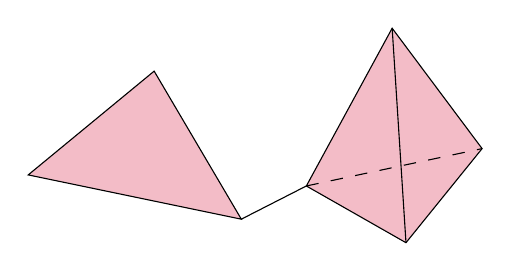
\begin{tikzpicture}[x=0.75pt,y=0.75pt,yscale=-1,xscale=1]
            \draw  [fill={rgb, 255:red, 232; green, 122; blue, 144 }  ,fill opacity=0.5 ] (121.89,134) -- (79.89,62.67) -- (19.22,112.67) -- cycle ;
            \draw    (121.89,134) -- (153.22,118) ;
            \draw  [fill={rgb, 255:red, 232; green, 122; blue, 144 }  ,fill opacity=0.5 ] (194.56,42) -- (153.22,118) -- (201.22,145.33) -- (237.89,100) -- cycle ;
            \draw  [dash pattern={on 4.5pt off 4.5pt}]  (153.22,118) -- (237.89,100) ;
            \draw    (194.56,42) -- (201.22,145.33) ;
        \end{tikzpicture}
        \hspace{7em}
        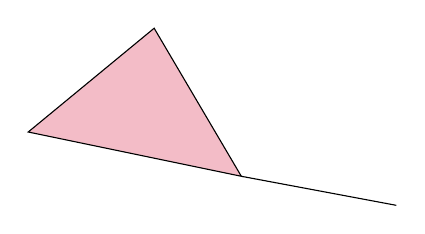
\begin{tikzpicture}[x=0.75pt,y=0.75pt,yscale=-1,xscale=1]
            \draw  [fill={rgb, 255:red, 232; green, 122; blue, 144 }  ,fill opacity=0.5 ] (121.89,134) -- (79.89,62.67) -- (19.22,112.67) -- cycle ;
            \draw    (121.89,134) -- (196.56,148) ;
        \end{tikzpicture}
    \end{center}

    \begin{Definition}[复形的维数]
        设 $ K $ 是一个复形, 称其\emph{维数}为
        \[
            \dim K:=\sup_{\sigma\in K}\dim\sigma.
        \]
        有限复形必是有限维的, 但反之不真.
    \end{Definition}

    对一个单形 $ \sigma^p\in\R^\N $, 可以从此出发构造复形
    \[
        K_{\sigma^p}:=\set{\tau : \tau\prec\sigma^p}
    \]
    和其边界复形
    \[
        \mathrm{Bd}\,K_{\sigma^p}=K_{\partial\sigma^p}:=K_{\sigma^p}\sm\set{\sigma}.
    \]
    更具体一些, 有复形的骨架的概念:

    \begin{Definition}[骨架]
        设 $ K $ 是一个复形, 称
        \[
            K^{(p)}:=\set{\sigma\in K : \dim\sigma\leqslant p}
        \]
        是 $ K $ 的\emph{$ p $维骨架}. 于是 $ K^{(p)} $ 也是一个复形, $ K^{(p)}\subset K $ 是 $ K $ 的一个子复形. 特别地, $ K^{(0)} $ 称作是 $ K $ 的\emph{顶点集}, 其中的元素称作 $ K $ 的\emph{顶点}.
    \end{Definition}

    直观上当 $ p=1 $ 时, 1维骨架就是直观上看起来的复形的 ``骨架'', 它只包含复形的0维子复形(即顶点)和1维子复形(即各边).

	设 $ K $ 是 $ \R^\N $ 的复形, 称
    \[
        \abs{K}=\bigcup_{\sigma\in K}\sigma
    \]
    是 $ K $ 的\emph{几何实现}或\emph{伴随多面体}. 此时 $ \abs{K} $ 成为 $ \R^\N $ 中的子集, 赋予拓扑 $ \CT_{\abs{K}} $ 是 $ \R^\N $ 上的子空间拓扑.

    \begin{Lemma}\label{lem:子复形几何实现的闭性}
        设 $ L $ 是 $ K $ 的子复形, 则 $ \abs{L} $ 是 $ \abs{K} $ 中的闭集.
    \end{Lemma}
    \begin{Proof}
        设 $ A\subset\abs{L} $ 是闭集, 对任意 $ \sigma\in K $, 有
        \[
            \sigma\cup\abs{L}=\bigcup_{\tau\prec\sigma,\tau\in L}\tau,
        \]
        故
        \[
            A\cap\sigma=\bigcup_{\tau\prec\sigma,\tau\in L}(A\cap\tau).
        \]
        而 $ A\cap\tau $ 是 $ \tau $ 中的闭集, 且 $ \tau\prec\sigma $, 故 $ A\cap\tau $ 是 $ \sigma $ 中的闭集, 进而 $ A\cap\sigma $ 也是 $ \sigma $ 中的闭集. 由此可知 $ A $ 是 $ \abs{K} $ 中的闭集.

        特别地, 取 $ A=\abs{L} $ 即可证明引理.\qed
    \end{Proof}

    由此可以说明在 $ \abs{K} $ 上的拓扑在一般情形下是弱于 Euclid 拓扑的, 即使它可以被嵌入有限维空间. 为此考虑复形
    \[
        K=\set{[m,m+1] : m\ne 0,\,m\in\Z}\cup\set{\Big[ \frac{1}{n+1},\frac{1}{n} \Big] : n\in\Z_+}\cup\Z\cup\set{\frac{1}{n} : n\in\Z_+}.
    \]
    则 $ \abs{K}=\R $, 且 $ L=\set{1/n : n\in\Z_+} $ 是 $ K $ 的子复形. 由引理~\ref{lem:子复形几何实现的闭性}~可知 $ \abs{L}=L $ 是 $ \abs{K} $ 中的闭集, 但在 $ \abs{K} $ 的 Euclid 拓扑下 $ \abs{L} $ 并不是闭集, 因它有聚点 $ 0\notin\abs{L} $.

	\begin{Definition}[可三角剖分空间]
        称拓扑空间 $ X $ \emph{可三角剖分}, 若存在复形 $ K $ 使得 $ X\cong\abs{K} $.
    \end{Definition}

    所有的光滑流形都可以被三角剖分, 一个例子是环面 $ \T^2 $ 可以被下图三角剖分:
    \begin{figure}[htbp]
        \centering
        \includegraphics[width=0.6\textwidth]{figures/Sec1_torus.png}
        \caption{$ \T^2 $ 的三角剖分}
    \end{figure}
    但需要注意的是下图的剖分方式并不是三角剖分, 因标注 $ \alpha $ 和 $ \beta $ 的两个三角形同时相交于点 $ A $ 和线 $ BC $, 它们不是公共面(\textit{因不连通}).
    \begin{figure}[htbp]
        \centering
        \includegraphics[width=0.2\textwidth]{figures/Sec1-2.png}
        \caption{一种不是三角剖分的 $ \T^2 $ 的剖分方式}
    \end{figure}

	\subsection{单纯映射}

	单纯复形范畴可以看作偏序范畴的一种, 考虑由真面诱导的偏序 $ \prec $, 那么 $ (K,\prec) $ 构成一个偏序集, 因此我们需要保持偏序结构的态射:

    \begin{Definition}[单纯映射]
        称 $ f : K\to L $ 是一个\emph{单纯映射}, 若对任意 $ \sigma\in K $ 都有 $ f(\sigma)\in L $, $ f $ 保持偏序关系, 即
        \[
            \tau\prec\sigma\Longrightarrow f(\tau)\prec f(\sigma),
        \]
        同时要求 $ \dim f(\sigma)\leqslant\dim\sigma $.
    \end{Definition}

    这与教材上的定义是等价的. $ \dim f(\sigma)\leqslant\dim\sigma $ 保证了 $ f $ 将 $ K $ 的顶点 $ K^{(0)} $ 映到 $ L $ 的顶点 $ L^{(0)} $. 单形本质上就可以看作是一些顶点的集合(由习题1-1保证). 于是单纯映射可以作为态射, 构成一个范畴 $ \category{SimComp} $, 称作是\emph{单纯复形范畴}.

    单纯映射 $ f : K\to L $ 诱导一个拓扑空间之间的映射 $ g_f $, 它满足
    \[
        g_f : \abs{K}\to\abs{L},\qquad x=\sum_{i=0}^pt_i\sigma_i\mapsto \sum_{i=0}^pt_if(\sigma_i),
    \]
    它可以看作是一系列形如 $ g_f|_\sigma : \sigma\mapsto\abs{L} $ 拼接起来的映射. 在拓扑空间范畴 $ \category{Top} $ 中, 我们当然希望 $ g_f $ 是连续的, 从而导出一个 $ \category{SimComp} $ 到 $ \category{Top} $ 的函子. 为此先证明以下引理:

    \begin{Lemma}
        $ h : \abs{K}\to X $ 连续当且仅当对任意 $ \sigma\in K $, 都有 $ h|_\sigma : \sigma\to X $ 连续.
    \end{Lemma}
    \begin{Proof}
        \textit{必要性.} 显然.

        \textit{充分性.} 任取 $ X $ 上的闭集 $ C $, 对任意 $ \sigma\in K $, 只需要证明 $ h^{-1}(C)\cap\sigma $ 是 $ \sigma $ 中的闭集即可. 而
        \[
            h^{-1}(C)\cap \sigma=(h|_\sigma)^{-1}(C)
        \]
        是闭的.\qed
    \end{Proof}

    由此得到:

    \begin{Proposition}
        $ F : K\mapsto\abs{K},\ f\mapsto g_f $ 给出一个 $ \category{SimComp} $ 到 $ \category{Top} $ 的函子.
    \end{Proposition}
    \begin{Proof}
        只需验证 $ F $ 的函子性, 首先 $ \id_K : K\to K $ 诱导出 $ F\id_K=\id_{\abs{K}} : \abs{K}\to\abs{K} $, 于是只需要证明图
        \begin{center}
            \begin{tikzcd}
                \abs{K} \arrow[r, "g_f"] \arrow[rd, "g_hg_f"'] & \abs{L} \arrow[d, "g_h"] \\
                                                               & \abs{M}                 
            \end{tikzcd}
        \end{center}
        交换即可. 这因
        \[
            g_{hf}(x)=\sum_{i=0}^pt_i(hf)(\sigma_i)=g_h\sum_{i=0}^pt_if(\sigma_i)=g_hg_f(x).
        \]\qed
    \end{Proof}

	对复形 $ K $, 其中的单形 $ \sigma=(\sigma_0,\dots,\sigma_p) $ 可以由顶点集 $ \set{\sigma_0,\dots,\sigma_p} $ 描述, 因此 $ K $ 在某种程度上可以由 $ K^{(0)} $ 描述.

    \begin{Definition}[抽象复形]
        设 $ S $ 是一个集合, 称 $ \CK\subset 2^S $ 是一个\emph{抽象复形}, 若
        \[
            \forall s\in\CK\,(t\subset s\Longrightarrow t\in\CK).
        \]
        此时的 $ s $ 即为抽象单形, $ \dim s=\abs{s}-1 $. 特别地, $ \dim\varnothing=-1 $. 类似可定义抽象复形的维数
        \[
            \dim\CK:=\sup_{s\in\CK}\dim s.
        \]
        对抽象复形, 也可以定义骨架 $ \CK^{(p)}:=\set{s\in\CK : \dim s\leqslant p} $.
    \end{Definition}

	\begin{Definition}[几何实现复形]
        称 $ K $ 是 $ \CK $ 的\emph{几何实现复形}, 若存在双射 $ f : K^{(0)}\to\CK^{(0)} $ 使得
        \[
            (v_0,\dots,v_p)\in K\Longleftrightarrow \set{f(v_0),\dots,f(v_p)}\in\CK.
        \]
    \end{Definition}

    抽象复形 $ \CK $ 的所有几何实现复形的伴随多面体都是分段线性同胚的, 因此之后我们不区分抽象复形和几何复形.

    \begin{Theorem}
        设 $ \CK^n $ 是 $ n $ 维有限抽象复形, 它必可在 $ \R^{2n+1} $ 上实现为几何复形.
    \end{Theorem}
    \begin{Proof}
        考虑循环曲线
        \[
            \varPhi : \R\to\R^{2n+1},\qquad t\mapsto (t,t^2,\dots,t^{2n+1}),
        \]
        断言对于互不相同的 $ t_0,\dots,t_{2n+1} $, 有 $ \varPhi(t_0),\dots,\varPhi(t_{2n+1}) $ 几何独立. 为此, 考虑
        \[
            \det[\varPhi(t_1)-\varPhi(t_0),\dots,\varPhi(t_{2n+1})-\varPhi(t_0)]=\mqty[t_1-t_0 & \cdots & t_{2n+1}-t_0 \\ \vdots & \ddots & \vdots \\ t_1^{2n+1}-t_0^{2n+1} & \cdots & t_{2n+1}^{2n+1}-t_0^{2n+1}]\ne 0
        \]
        即得断言.

        令 $ \CK^{(0)}=\set{s_1,\dots,s_N}\sm\set{\varnothing} $, 几何复形 $ K $ 构造如下:
        \[
            \CK^{0}\ni s_i\longleftrightarrow\varPhi(i)\in K^{(0)},
        \] 
        则 $ s=\set{s_{i_1},\dots,s_{i_p}}\in\CK $ 当且仅当 $ (\varPhi(i_1),\dots,\varPhi(i_p))\in K $, 其中 $ p\leqslant n $. 下面证明如此构造的 $ K $ 是一个几何复形, 定义的第一条显然满足, 只需证明任意两个单形的交或者非空, 或者是公共面即可.

        任取 $ \sigma^p,\sigma^q\in K $, 设它们有 $ r $ 个公共顶点, 则 $ \sigma^p $ 和 $ \sigma^q $ 共有 $ p+1+q+1-r $ 个不同的顶点, 而
        \[
            p+q+2-r\leqslant 2n+2-r<2n+2,
        \]
        于是这些顶点几何独立, 它们确定了一个 $ p+q+1-r $ 维单形 $ \gamma $, 满足 $ \sigma^p\prec\gamma $, $ \sigma^q\prec\gamma $. 因此由单形的定义可知它们的交或者非空, 或者是公共面.\qed
    \end{Proof}

    \begin{Corollary}
        设 $ K $ 是有限复形, 且 $ \dim K=n $, 则一定存在嵌入 $ \abs{K}\hookrightarrow\R^{2n+1} $.
    \end{Corollary}

    但是将上一推论的嵌入从 $ \R^{2n+1} $ 改为 $ \R^{2n} $ 后就不再成立了. 例如 $ K_{\sigma^{2n+2}}^{(n)} $ 就不能嵌入 $ \R^{2n} $. 最简单的情形, 令 $ n=1 $, 此时 $ K_{\sigma^4}^{(1)} $ 即为下图:
    \begin{figure}[htbp]
        \centering
        \includegraphics[width=0.2\textwidth]{figures/Sec2-1.png}
        \caption{$ K_{\sigma^4}^{(1)}=K_{5,5} $}
    \end{figure}
    它就是图 $ K_{5,5} $, 是一类不可平面化的图, 于是它不能嵌入 $ \R^2 $.

	\subsection{单纯同调群}

	对复形的定向无非是对顶点的排序, 而排序本质上只有两种, 即由偶置换确定的同构类. 对 $ \sigma $ 的顶点集 $ \set{v_0,\dots, v_p} $, 定义它在偶置换下的同构类为 $ [v_0,\dots,v_p] $, 就称它是复形 $ \sigma $ 的一个\emph{定向}.

    特别地, 约定 0 维情形下, $ [a_0] $ 与 $ -[a_0] $ 是两种不同的定向.

    \begin{figure}[htbp]
        \centering
        \includegraphics[width=0.6\textwidth]{figures/Sec3-1.png}
        \caption{低维复形的定向}
    \end{figure}

    \begin{Definition}[定向复形]
        称 $ K $ 是一个\emph{定向复形}, 若 $ \forall \sigma\in K $, $ \sigma $ 是有定向的. 并记
        \[
            S_p^+(K):=\set{\sigma\in K : \dim\sigma=p},\qquad S_p(K)=\set{\pm\sigma : \sigma\in S_p^+(K)}.
        \]
    \end{Definition}

    \begin{Theorem}
        由 $ S_p^+(K) $ 作为生成元可以生成一个自由 Abel 群, 记作
        \[
            C_p(K):=\set{\sum_{\sigma\in S_p^+(K)}n_\sigma\sigma},
        \]
        并要求求和为有限和.
    \end{Theorem}
    \begin{Proof}
        考虑映射 $ c_p : S_p(K)\to\Z $, 其中 $ c_p $ 仅在 $ S_p(K) $ 中有限个元素上取非零值, 且 $ \forall\sigma\in S_p(K) $ 都有 $ c_p(-\sigma)=-c_p(\sigma) $. 称 $ c_p $ 是一个\emph{$ p $--链}. 取
        \[
            C_p(K)=\set{c_p : S_p(K)\to\Z},
        \]
        在它上面定义加法
        \[
            (c_p+c_p')(\sigma):=c_p(\sigma)+c_p'(\sigma),
        \]
        则 $ (C_p(K),+) $ 是一个 Abel 群, 其中的零元 $ 0 : S_p(K)\to\Z $, $ \sigma\mapsto 0 $, $ c_p $ 的逆 $ (-c_p)(\sigma):=-c_p(\sigma) $.

        接下来证明它是由 $ S_p^+(K) $ 生成的自由 Abel 群. 我们需要做一点说明, 对 $ \sigma\in S_p^+(K) $, 定义
        \[
            c_p^\sigma(\tau)=\begin{cases}
                \pm 1 & ,\tau=\pm\sigma \\ 0 & ,\tau\ne\pm\sigma
            \end{cases}
        \]
        则 $ \set{c_p^\sigma}_{\sigma\in S_p^+(K)} $ 与 $ S_p^+(K) $ 之间可以建立 1--1 对应, 于是可以用 $ \sigma $ 替代 $ c_p^{\sigma} $. 对 $ \forall c_p\in C_p(K) $, $ \forall \sigma\in S_p^+(K) $, 记 $ c_p(\sigma)=n_\sigma $, 那么构造的
        \[
            c_p'=\sum_{\sigma\in S_p^+(K)}n_\sigma c_p^\sigma=\sum_{\sigma\in S_p^+(K)}n_\sigma\sigma
        \]
        自然是有限和. 断言 $ c_p'=c_p $.

        为此, 对任意 $ \tau\in S_p(K) $, 考虑
        \[
            c_p'(\tau)=\sum_{\sigma\in S_p^+(K)}n_\sigma c_p^\sigma(\tau)\stackrel{\tau=\pm\sigma}{=}\pm n_\sigma=c_p(\pm\sigma)=c_p(\tau).
        \]
        再说明唯一性, 令 $ c_p=\sum_{\sigma\in S_p^+(K)}n_\sigma \sigma=\sum_{\sigma\in S_p^+(K)}n_\sigma'\sigma $, 则
        \[
            \sum_{\sigma\in S_p^+(K)}(n_\sigma-n_\sigma')\sigma=0_p.
        \]
        代入 $ \tau=\pm\sigma $ 得到
        \[
            \sum_{\sigma\in S_p^+(K)}(n_\sigma-n_\sigma')c_p^\sigma(\tau)=\pm(n_\sigma-n_\sigma')=0_p(\tau)=0,
        \]
        即 $ n_\sigma=n_\sigma' $, 断言得证.\qed
    \end{Proof}

	\begin{figure}[htbp]
		\centering
        \includegraphics[width=0.3\linewidth]{figures/Sec3-2.png}
		\caption{一个 2 维定向复形的例子}
	\end{figure}

	考虑以上 2 维复形的边界, 计算 $ \partial[v_0,v_1,v_2] $ 得到
    \[
            \partial[v_0,v_1,v_2]=[v_0,v_1]+[v_1,v_2]+[v_2,v_0]=[v_0,v_1]-[v_0,v_2]+[v_1,v_2].
    \]
    并且注意到边界中的每一项符号与缺少的顶点标号有关.

	\begin{figure}[htbp]
		\centering
        \includegraphics[width=0.3\linewidth]{figures/Sec3-3.png}
        \caption{一个 3 维定向复形的例子}
	\end{figure}

	再考虑 3 维复形的边界: 这里所有 2 维面的定向都使用右手法则来确定. 计算 $ \partial[v_0,v_1,v_2,v_3] $ 得到
    \[
        \begin{aligned}
            \partial[v_0,v_1,v_2,v_3]& =[v_0,v_2,v_1]+[v_0,v_1,v_3]+[v_1,v_2,v_3]+[v_0,v_3,v_2]\\
            & =-[v_0,v_1,v_2]+[v_0,v_1,v_3]-[v_0,v_2,v_3]+[v_1,v_2,v_3].
        \end{aligned}
    \]
    同样地, 注意到边界中的每一项符号都与缺少的顶点标号有关.

	由此可以归纳得到,
    \[
        \partial[v_0,\dots,v_p]=\sum_{k=0}^p(-1)^k[v_0,\dots,\hat{v}_k,\dots,v_p],
    \]
    其中 $ \hat{v_k} $ 表示缺少这一项.

	\begin{Definition}[边缘算子]
        称
        \[
            \partial : C_p(K)\to C_{p-1}(K),\qquad c_p=\sum_{\sigma\in S_p^+(K)}n_\sigma\sigma\mapsto\sum_{\sigma\in S_p^+(K)}n_\sigma\partial\sigma
        \]
        是 $ C_p(K) $ 上的\emph{边缘算子}, 有时为了强调也记作 $ \partial_p $. 它是 $ C_p(K) $ 到 $ C_{p-1}(K) $ 的群同态, 其中 $ \partial\sigma $ 如下定义: 对 $ \sigma=[v_0,\dots,v_p] $, 有
        \[
            \partial[v_0,\dots,v_p]=\sum_{k=0}^p(-1)^k[v_0,\dots,\hat{v}_k,\dots,v_p].
        \]
    \end{Definition}

    \begin{Proposition}
        $ \partial^2=0 $. (\textit{严格地讲, 应该写成 $ \partial_{p-1}\partial_p=0 $})
    \end{Proposition}
    \begin{Proof}
        任取 $ \sigma=[v_0,\dots,v_p] $, 计算
        \[
            \begin{aligned}
                \partial^2\sigma&=\partial\left( \sum_{k=0}^p(-1)^k[v_0,\dots,\hat{v}_k,\dots,v_p] \right)\\
                &=\sum_{j<k}(-1)^k(-1)^j[\dots,\hat{v}_j,\dots,\hat{v}_k,\dots]+\sum_{j>k}(-1)^k(-1)^{j-1}[\dots,\hat{v}_k,\dots,\hat{v}_j,\dots]\\
                &=\sum_{j<k}(-1)^{k+j}[\dots,\hat{v}_j,\dots,\hat{v}_k,\dots]+\sum_{j<k}(-1)^{k+j-1}[\dots,\hat{v}_j,\dots,\hat{v}_k,\dots]\\
                &=0.
            \end{aligned}
        \]
        于是命题得证.\qed
    \end{Proof}

	\begin{Definition}[同调群]
        对链复形 $ \mathcal{C}(K)=\set{(C_p(K),\partial_p} $,
        \begin{center}
            \begin{tikzcd}
                {} \arrow[r, "\partial_{p+1}"] & C_p(K) \arrow[r, "\partial_p"] & C_{p-1}(K) \arrow[r, "\partial_{p-1}"] & \cdots \arrow[r, "\partial_2"] & C_1(K) \arrow[r, "\partial_1"] & C_0(K) \arrow[r, "\partial_0"] & {}
            \end{tikzcd}
        \end{center}
        对 $ \partial_p : C_p(K)\to C_{p-1}(K) $, 称
        \begin{enumerate}[(1)]
            \item $ Z_p(K):=\ker\partial_p=\set{c_p\in C_p(K) : \partial c_p=0} $ 是 $ K $ 的 \emph{$ p $ 维闭链群};
            \item $ B_p(K):=\im\partial_{p+1}=\set{\partial c_{p+1}\in C_p(K) : c_{p+1}\in C_{p+1}(K)} $ 是 $ K $ 的 \emph{$ p $ 维边缘链群}.
        \end{enumerate}
        满足 $ B_p(K)\norsub Z_p(K) $, 且 $ B_p(K) $ 和 $ Z_p(K) $ 仍是自由 Abel 群. 称
        \[
            H_p(K)=\ker\partial_p/\im\partial_{p+1}=Z_p(K)/B_p(K)
        \]
        是 $ K $ 的\emph{$ p $ 阶同调群}.
    \end{Definition}

	在 $ Z_p(K) $ 上可以定义等价关系:
    \[
        \begin{aligned}
            z_p\sim z_p' & \Longleftrightarrow z_p+B_p(K)=z_p'+B_p(K)\\
            & \Longleftrightarrow z_p-z_p'+B_p(K)=0\Longleftrightarrow \exists d\in C_{p+1}(K)\,(\partial d=z_p-z_p'),
        \end{aligned}
    \]
    这一等价关系称作\emph{同调关系}, 确定的等价类 $ \bar{z}_p $ 称作\emph{同调类}. 它可以不局限于闭链群, 例如在 $ C_p(K) $ 上同样可以定义
    \[
        c_p\sim c_p'\Longleftrightarrow \exists d\in C_{p+1}(K)\,(\partial d=c_p-c_p').
    \]
    特别地, 若 $ \partial d=c_p $, 则 $ c_p\sim 0 $.

    \begin{Example}
        考虑以下的 2 维复形, 约定每一个 2 维单形的定向都是逆时针.
		\begin{figure}[htbp]
			\centering
        	\includegraphics[width=0.3\linewidth]{figures/Sec3-4.png}
		\end{figure}

		取
    	\[
    	        \begin{aligned}
    	            z_1&=[v_0,v_1]+[v_1,v_2]+[v_2,v_0]\in C_1(K)\\
    	            z_2&=[v_3,v_4]+[v_4,v_5]+[v_5,v_3]\in C_1(K),
    	        \end{aligned}
    	\]
    
    	计算可得
    	\[
    	        \partial z_1=\partial z_2=0,
    	\]
    	于是 $ z_1,z_2\in Z_1(K) $. 而
    	\[
    	    \partial\Big(\sum_{\sigma\in K^{(2)}\sm K^{(1)}}\sigma\Big)=z_1-z_2, 
    	\]
    	于是由同调关系的定义可知 $ z_1\sim z_2 $.
    \end{Example}

	将 $ \partial_p $ 限制到 $ \im\partial_p $ 上之后可知
    \[
        \partial_p : C_p(K)\twoheadrightarrow\im\partial_p=B_{p-1}(K)
    \]
    是一个满同态. 于是由同态基本定理可知 $ C_p(K)/\ker\partial_p\simeq\im\partial_p $.~

    对复形 $ K $, $ v,w\in K^{(0)} $, 则 $ v,w\in C_0(K) $. 于是由同调关系的定义可知
    \[
        v\sim w\Longleftrightarrow\exists d\in C_1(K)\,(\partial d=w-v).
    \]
    在直观上, $ v\sim w $ 即是存在一列 $ \set{v_i}_{i=0}^n $ 满足 $ v_0=v $, $ v_n=w $ 使得 $ v $ 与 $ w $ 可以经由 $ [v_i,v_{i+1}] $ 相连.

    \begin{figure}
        \centering
        \includegraphics[width=0.4\linewidth]{figures/Sec3-5.png}
    \end{figure}

    于是同调关系可以对 $ K^{(0)} $ 分类, 以 $ \bar{v}:=\set{w\sim v : w\in K^{(0)}} $ 记 $ v $ 所在的等价类, 则
    \[
        K=\bigcup_{\bar{v}\in K^{(0)}/\sim}K_{\bar{v}}=\bigcup_{\bar{v}\in K^{(0)}/\sim}\set{(v_0,\dots,v_p)\in K : \set{v_0,\dots,v_p}\subset\bar{v}}.
    \]
    进一步, 其几何实现
    \[
        \abs{K}=\bigcup_{\bar{v}\in K^{(0)}/\sim}\abs{K_{\bar{v}}},
    \]
    且 $ \abs{K_{\bar{v}}} $ 是道路连通的. 此时也称 $ K_{\bar{v}} $ 是道路连通的.

    \begin{Theorem}
        对复形 $ K $, $ H_p(K)=\bigoplus_{\bar{v}\in K^{(0)}/\sim}H_p(K_{\bar{v}}) $, 即计算同调群只需分别计算各个道路连通分支的同调群即可.
    \end{Theorem}
    \begin{Proof}
        首先 $ C_p(K)=\bigoplus_{\bar{v}\in K^{(0)}/\sim}C_p(K_{\bar{v}}) $, 只需证明
        \[
            Z_p(K)=\bigoplus_{\bar{v}\in K^{(0)}/\sim}Z_p(K_{\bar{v}}),\qquad B_p(K)=\bigoplus_{\bar{v}\in K^{(0)}/\sim}B_p(K_{\bar{v}})
        \]
        即可. 注意到
        \[
            z_p\in Z_p(K)\norsub C_p(K)=\bigoplus_{\bar{v}\in K^{(0)}/\sim}C_p(K_{\bar{v}}),
        \]
        这导出 $ z_p=\sum_{\bar{v}\in K^{(0)}/\sim}c_p^{\bar{v}} $. 于是
        \[
            0=\partial z_p=\sum_{\bar{v}\in K^{(0)}/\sim}\partial c_p^{\bar{v}}
        \]
        导出 $ \partial c_p^{\bar{v}}=0 $. $ B_p(K) $ 的情形类似可证.\qed
    \end{Proof}

    让我们做些计算! 设 $ X $ 是一个拓扑空间, $ H_0(X) $ 是其 0 阶同调群. 取 $ C_0(X) $, 它就是 $ X $ 中点的形式和. 考虑边缘函数
    \[
        \partial : C_0(X)\to 0
    \]
    的核, $ \ker\partial $ 即为整个空间 $ C_0(X) $, 这意味着每一个点都是一个 ``环''. 而 $ [b]-[a]=0 $ 当且仅当存在一个 1 维链连结 $ a $ 和 $ b $, 于是这自然导向道路连通空间.

    \begin{Proposition}\label{prop:道路连通复形的0阶同调群}
        设 $ K $ 是道路连通复形, 则 $ H_0(K)=\Z $.
    \end{Proposition}
    \begin{Proof}
        设 $ v\in K^{(0)} $, 则 $ \forall w\in K^{(0)} $, 因 $ K $ 是道路连通的, 于是
        \[
            v\sim w\Longleftrightarrow v+B_0(K)=\set{v}=\set{w}=w+B_0(K),
        \]
        则对任意 $ \alpha=c_0+B_0(K)\in H_0(K) $, 都有
        \[
            c_0+B_0(K)=\sum_{v\in K^{(0)}}n_vv+B_0(K)\stackrel{\text{固定}\,v'}{=}nv'+B_0(K)=n\set{v'},
        \]
        故 $ H_0(K)=\Z_{\set{v'}}=\set{n\set{v'} : n\in\Z} $. 断言 $ \set{v'} $ 是一个无限阶元.

        为此, 令 $ n\set{v'}=0 $, 也即 $ nv'+B_0(K)=0 $, 则
        \[
            \exists c_1\in C_1(K)\,(\partial c_1=nv'),
        \]
        另一方面
        \[
            c_1=\sum n_{ij}[v_i,v_j],\qquad\partial[v_i,v_j]=v_j-v_i,
        \]
        故 $ \partial c_1=\sum_{v\in K^{(0)}}n_vv $ 中的系数和 $ \sum_{v\in K^{(0)}}n_v=0 $, 又由 $ \partial c_1=\sum_{v\in K^{(0)}}n_vv=nv' $ 可知
        \[
            n_v=\begin{cases}
                n & ,v=v' \\ 0 & ,v\ne v'
            \end{cases}
        \]
        而系数和为零, 于是只能 $ n=0 $, 此即 $ H_0(K)=\Z $.\qed
    \end{Proof}

    \begin{Corollary}
        $ \abs{K} $ 是道路连通的当且仅当 $ H_0(K)=\Z $.
    \end{Corollary}

	\subsection{2 维闭曲面的同调群}

	\begin{Example}[2 维闭曲面的代数表示]
        2 维闭曲面一共两类, 一类是可定向的:
        \begin{figure}[htbp]
            \centering
            \includegraphics[width=0.7\linewidth]{figures/Sec3-6.png}
            \caption{可定向的 2 维闭曲面}
        \end{figure}
        ~\\其中 $ \sharp $ 表示连通和. 它在两个流形中各挖去一个球, 并将球面边界粘贴在一起得到. 而不可定向的一类为
        \[
            \mathbb{RP}^2,\ \mathbb{RP}^2\sharp\mathbb{RP}^2,\ \cdots,\ \mathbb{RP}^2\sharp\cdots\sharp\mathbb{RP}^2,\cdots,
        \]
        其中 Klein 瓶实际上就是 $ \mathbb{RP}^2\sharp\mathbb{RP}^2 $. 由此, 2 维闭曲面的全体可以看作代数系
        \[
            \lrangle{\S^2,\T^2,\mathbb{RP}^2;\sharp}.
        \]
        (\textit{当然, 这里需要证明 $ \sharp $ 的确是一个代数运算. 首先对于可定向曲面, 亏格 $ g $ 就是它的拓扑不变量. 对于不可定向曲面, 无论做了多少次连通和, 它永远可以通过连续变形构成一个定向曲面和一个 M\"obius 带的形式.})
        \begin{figure}[htbp]
            \centering
            \includegraphics[width=0.7\linewidth]{figures/Sec3-7.png}
            \caption{一个 $ \mathbb{RP}^2 $ 和 $ \mathbb{RP}^2 $ 作连通和的例子}
        \end{figure}
    \end{Example}

	为了应用所谓的 push off 方法, 我们约定所有的 2 维单形定向均为逆时针定向. 这有利于我们将复形推到它的边界上进行讨论.

    \begin{Lemma}\label{lem:推到边界复形}
        设 $ K $ 是一个闭曲面, 则
        \begin{enumerate}[(1)]
            \item 对 $ z_1\in Z_1(K) $, 存在 $ z_1'\in Z_1(\Bd K) $ 使得 $ z_1\sim z_1' $;
            \item 对 $ d\in Z_2(K) $ 使得 $ \partial d\in C_1(\Bd K) $, 有 $ d=l\left(\sum_{\dim\sigma=2}\sigma\right) $.
        \end{enumerate}
    \end{Lemma}
    \begin{Proof}
        (1) 因 $ z_1\in Z_1(K)\norsub C_1(K) $, $ z_1=\sum n_{ij}[v_i,v_j] $, 若一个非边界的 $ [v_i,v_j] $ 使得 $ n_{ij}\ne 0 $, 则可以取到一个使得 $ [v_i,v_j] $ 系数为负的 2 维复形 $ \sigma_1 $:
        \begin{figure}[h]
            \centering
            \includegraphics[width=0.25\linewidth]{figures/Sec3-8.png}
        \end{figure}
        
        此时
        \[
            \partial(n_{ij}\sigma_1)=n_{ij}\partial\sigma_1=-n_{ij}[v_i,v_j]+\cdots,
        \]
        注意到取边界并不影响 $ B_1(K) $, 于是
        \[
            z_1+B_1(K)=z_1+\partial(n_{ij}\sigma_1)+B_1(K)=\cdots=z_1'+B_1(K)
        \]
        使得 $ z_1\in Z_1(\Bd K) $.

        (2) 由 $ d\in Z_2(K) $ 可知
        \[
            d=\sum_{\dim\sigma=2}n_\sigma\sigma,\qquad\partial d\in Z_1(\Bd K),
        \]
        由此, 考虑非边界上的 1 维边, 如下图所示
        \begin{figure}[htbp]
            \centering
            \includegraphics[width=0.25\linewidth]{figures/Sec3-9.png}
        \end{figure}
        ~\\于是对粉色边, 应当有 $ n_\sigma=n_{\sigma'} $, 再对蓝色边讨论, 有 $ n_{\sigma'}=n_{\sigma''} $, 由此进行下去可知 $ d $ 中所有的 $ n_\sigma $ 都相同.\qed
    \end{Proof}

    \begin{Example}[$ \T^2 $ 的同调群]
        考虑 $ \T^2 $ 的三角剖分
		\begin{figure}[htbp]
    		\centering
        	\includegraphics[width=0.25\linewidth]{figures/Sec3-10.png}
    	\end{figure}

		对 $ p<0 $ 和 $ p>2 $ 自然有 $ H_p(\T^2)=0 $.
    
    因 $ \T^2 $ 道路连通, 由命题~\ref{prop:道路连通复形的0阶同调群}~可知 $ H_0(\T^2)=\Z $, 于是只需要计算 $ H_1(\T^2) $ 和 $ H_2(\T^2) $

    对 $ \alpha\in H_1(\T^2) $, 有
    \[
        \alpha=z_1+B_1(K)=\set{z_1}, 
    \]
    由引理~\ref{lem:推到边界复形}~的(1)可知存在 $ z_1'\in Z_1(\Bd K) $ 使得 $ z_1\sim z_1' $. 而
    \[
        \Bd K=\set{[a,b],[b,c],[c,a],[a,d],[d,e],[e,a]}.
    \]
    设
    \[
        z_1'=\sum_{i,j}n_{i,j}[i,j],
    \]
    令
    \[
        \begin{aligned}
            0&=\partial z_1'\\
            &=(-n_{ab}+n_{ca}-n_{ad}+n_{ea})a+(n_{ab}-b_{bc})b+(n_{bc}-n_{ca})c+(n_{ad}-n_{de})d+(n_{de}-n_{ea})e\\
        \end{aligned}
    \]
    即
    \[
        n_{ab}=n_{bc}=n_{ca}=n,\qquad n_{ad}=n_{de}=n_{ea}=m.
    \]

    为此, 记 $ w=[a,b]+[b,c]+[c,a] $, $ z=[a,d]+[d,e]+[e,a] $, 则
    \[
        \set{z_1}=\set{z_1'}=\set{nw+mz}=nw+mz+B_1(K)=n\set{w}+m\set{z}+B_1(K),
    \]
    故 $ H_1(\T^2)=\Z_{\set{w}}+\Z_{\set{z}} $. 下面证明这一和为直和, 且 $ \set{w} $ 和 $ \set{z} $ 都是无限阶元.

    令 $ n\set{w}+m\set{z}=0 $, 则
    \[
        \begin{aligned}
            nw+mz+B_1(K)=0& \Longleftrightarrow \exists d\in C_2(K)\,(\partial d=nw+mz\in Z_1(\Bd K))\\
            & \Longrightarrow d=l\Big( \sum_{\dim\sigma=2}\sigma \Big).
        \end{aligned}
    \]
    其中第二行的推出由引理~\ref{lem:推到边界复形}~的(2)得到. 此时 $ \partial\left(\sum_{\dim\sigma=2}\sigma\right)=0 $ (\textit{在三角剖分图中标注出定向即可看出}), 即 $ \partial d=0 $, 从而 $ nw+mz=0\in Z_1(\Bd K) $, 且 $ n=m=0 $. 故
    \[
        H_1(\T^2)=\Z\oplus\Z.
    \]

    再计算 $ H_2(\T^2) $, 注意到 $ C_3(\T^2)=0 $, 故 $ B_2(\T^2)=0 $, 故 $ H_2(\T^2)=Z_2(\T^2) $. 对 $ \alpha=z_2+B_2(K)=z_2\in Z_2(\T^2) $, 有
    \[
        \begin{aligned}
            \partial z_2=0 & \Longrightarrow \partial z_2\in Z_1(\Bd K)\\
            & \Longrightarrow z_2=l\Big( \sum_{\dim\sigma=2}\sigma \Big)\\
            & \Longrightarrow H_2(\T^2)=\Z_{\left(\sum_{\dim\sigma=2}\sigma\right)}\cong\Z.
        \end{aligned}
    \]
    同样地, 第二行的推出由引理~\ref{lem:推到边界复形}~的(2)得到.

	由此, 我们得到环面 $ \T^2 $ 的同调群如下:
	\[
		H_p(\T^2)=\begin{cases}
			\Z & ,p=0,2\\ \Z\oplus\Z & ,p=1 \\ 0 &,\text{其他}
		\end{cases}
	\]
    \end{Example}

	\begin{Example}[Klein 瓶的同调群]
		Klein 瓶 $ S $ 的三角剖分如下图所示:
		\begin{figure}[htbp]
			\centering
			\includegraphics[width=0.25\linewidth]{figures/Sec3-11.png}
		\end{figure}
		
		类似地记
		\[
			w=[a,b]+[b,c]+[c,a],\qquad z=[a,d]+[d,e]+[e,a],
		\]
		类似于 $ \T^2 $ 的计算方法, 对 $ \set{z_1}=z_1+B_1(S)=z_1'+B_1(S) $, 其中 $ z_1'\in Z_1(\Bd S) $, 有
		\[
			\set{z_1'}=mw+nz+B_1(S)=m\set{w}+n\set{z},
		\]
		也即 $ H_1(S)=\Z_{\set{w}}+\Z_{\set{z}} $.

		令 $ m\set{w}+n\set{z}=0 $, 则
		\[
			\begin{aligned}
				mw+nz+B_1(S)=0&\Longleftrightarrow \exists d\in C_2(S)\,(\partial d=mw+nz\in Z_1(S))\\
				&\Longrightarrow d=l\Big(\sum_{\dim\sigma=2}\sigma\Big),
			\end{aligned}
		\]
		此时 $ \partial d=2lz $, 记 $ 2lz=mw+nz=0 $, 这意味着 $ \set{z} $ 是 2 阶元. 从而
		\[
			H_1(S)=\Z\oplus(\Z/2\Z).
		\]

		2 阶同调群的情形, 我们只需要注意到对唯一的 2 维单形 $ d $ 有 $ \partial d\ne 0 $ 即可得到 $ H_2(S)=0 $.

		由此, 我们得到 Klein 瓶的同调群如下:
		\[
			H_p(S)=\begin{cases}
				\Z & ,p=0\\ \Z\oplus(\Z/2\Z) & ,p=1 \\ 0 &,\text{其他}
			\end{cases}
		\]
	\end{Example}

	\subsection{约化同调}

	对单纯复形 $ K $ 的链复形
	\begin{center}
		\begin{tikzcd}
			{} \arrow[r, "\partial_{p+1}"] & C_p(K) \arrow[r, "\partial_p"] & C_{p-1}(K) \arrow[r, "\partial_{p-1}"] & \cdots \arrow[r, "\partial_2"] & C_1(K) \arrow[r, "\partial_1"] & C_0(K) \arrow[r, "\partial_0"] & {}
		\end{tikzcd}
	\end{center}
	它有增广链复形
	\begin{center}
		\begin{tikzcd}
			{} \arrow[r, "\partial"] & C_p(K) \arrow[r, "\partial"] & \cdots \arrow[r, "\partial"] & C_1(K) \arrow[r, "\partial"] & C_0(K) \arrow[r, "\varepsilon"] & \mathbb{Z} \arrow[r] & 0
		\end{tikzcd}
	\end{center}
	为了使得 $ \varepsilon\circ\partial=0 $, 只需要将 $ v\in C_0(K) $ 映到 $ \varepsilon(v)=1 $ 即可. 这由
	\[
		\varepsilon\partial[v_1,v_0]=\varepsilon(v_1)-\varepsilon(v_0)=0
	\]
	即可验证. 而对抽象复形 $ K $, 由于 $ \set{n\emptyset : n\in\Z}=C_{-1}(K)\cong\Z $ 的存在, 它与几何复形的增广链复形相同.

	\begin{Definition}[约化同调]
		称增广链复形导出的同调群 $ \tilde{H}_i(K) $ 是\emph{约化同调群}, 当 $ i>0 $ 时
		\[
			\tilde{H}_i(K)=H_i(K),
		\]
		而 $ i=0 $ 时 $ \tilde{H}_0(K)=\ker\varepsilon/\im\partial_1 $, 这里 $ \ker\varepsilon\leqslant C_0(K) $.
	\end{Definition}

	\begin{Proposition}
		$ H_0(K)\cong\tilde{H}_0(K)\oplus\Z $.
	\end{Proposition}
	\begin{Proof}
		设 $ K=\coprod_{i}K_i $, 其中 $ K_i $ 是 $ K $ 的道路连通分支. 任取 $ v_i\in K_i^{(0)} $, 有
		\[
			H_0(K)\cong\bigoplus_{i}\Z_{\set{v_i}}\cong\bigoplus_{i}\Z.
		\]
		考虑约化同调群 $ \tilde{H}_0(K) $, 设 $ \set{z_0}=z_0+\im\partial_1\in\tilde{H}_0(K) $, 其中 $ z_0\in\ker\varepsilon $.

		将 $ z_0+\im\partial_1 $ 在 $ C_0(K) $ 中观察得到
		\[
			z_0+\im\partial_1=\sum_{i}n_iv_i+\im\partial_1,
		\]
		在 $ \ker\varepsilon $ 中观察, 得到
		\[
			0=\varepsilon z_0=\sum_{i}n_i\Longrightarrow n_0=-\sum_{i\ne 0}n_i,
		\]
		由此
		\[
			\tilde{H}_0(K)=\bigoplus_{i\ne 0}\Z_{\set{v_i-v_0}}.
		\]
		令 $ \sum_{i\ne 0}n_i\set{v_i-v_0}=0\in\tilde{H}_0(K) $, 即 $ \sum_{i\ne 0}n_i(v_i-v_0)+\im\partial_1 $, 故存在 $ d=\sum n_uv[u,v]\in C_1(K) $ 使得
		\[
			\sum n_vv=\sum_{i\ne 0}n_i(v_i-v_0).
		\]
		这里 $ \sum n_v=0 $, 因注意到 $ \partial n_{uv}[u,v]=n_{uv}v-n_{uv}u $ 中点的系数总是一正一负交替出现, 比较上式两侧系数可知 $ n_i=0 $.\qed
	\end{Proof}

	\begin{Definition}[锥]
		设 $ K $ 是一个复形, $ v\in\R^\N $. 对任意 $ \sigma=(v_0,\dots,v_p)\in K $, 若 $ v,v_0,\dots,v_p $ 几何独立, 则它确定一个单形
		\[
			v*\sigma:=(v,v_0,\dots,v_p),
		\]
		它的定向由 $ [v,\sigma]:=[v,v_0,\dots,v_p] $ 确定. 由此得到一个复形
		\[
			v*K=K\cup\set{v}\cup\bigcup_{\sigma\in K}v*\sigma,
		\]
		称作在 $ v $ 处的\emph{锥}.
	\end{Definition}

	\begin{figure}[htbp]
		\centering
		\includegraphics[width=0.2\linewidth]{figures/Sec3-12.png}
		\caption{一个 2 维复形 $ K $ 与点 $ v $ 形成的锥}
	\end{figure}

	从几何上来看, 容易得到 $ \abs{v*K}\cong\mathrm{pt} $.

	\begin{Lemma}
		设 $ c $ 是 $ K $ 的单形, 则
		\[
			\partial[v,c]=\begin{cases}
				c-[v,\partial c] & ,\dim c>0\\
				c-\varepsilon(c)v & ,\dim c=0
			\end{cases}
		\]
	\end{Lemma}
	\begin{Proof}
		计算 $ v*K $ 的约化同调 $ \tilde{H}_p(v*K) $, 考虑
		\[
			c_{p+1}=c_1+c_2\in C_{p+1}(K),\qquad c_1\in C_{p+1}(K),\quad c_2=\sum_{\sigma\in K,\dim\sigma=p}n_\sigma(v*\sigma)=\left[ v,\sum_{\sigma\in K,\dim\sigma=p}n_\sigma\sigma \right]
		\]
		对 $ p>0 $, 有
		\[
			\begin{aligned}
				\partial[v,v_0,\dots,v_p]&=[v_0,\dots,v_p]+\sum_{i=0}^p(-1)^{i+1}[v,v_0,\dots,\hat{v}_i,\dots,v_p]\\
				&=[v_0,\dots,v_p]-\sum_{i=0}^p(-1)^i[v,v_0,\dots,\hat{v}_i,\dots,v_p]\\
				&=[v_0,\dots,v_p]-\left[ v,\sum_{i=0}^p[v,v_0,\dots,\hat{v}_i,\dots,v_p] \right]\\
				&=\sigma-[v,\partial\sigma].
			\end{aligned}
		\]
		对 $ p=0 $, 有 $ \partial[v,v_0]=v_0-v $.\qed
	\end{Proof}

	\begin{Theorem}
		锥 $ v*K $ 是零调的, 即 $ \tilde{H}_p(v*K)=0 $.
	\end{Theorem}
	\begin{Proof}
		对 $ p\leqslant 0 $ 和 $ p>\dim K $, 显然 $ \tilde{H}_p(K)=0 $.

		对 $ 1\leqslant p\leqslant\dim K $, 取 $ z\in C_p(v*K) $ 满足 $ \partial z=0 $, 即 $ z\in Z_p(v*K) $. 记 $ z=c_1+c_2 $, 其中 $ c_1\in C_p(K) $ 被 $ K $ 承载, $ c_2=[v,c_2'] $ 被 $ v*K $ 承载. 计算
		\[
			0=\partial z=\partial c_1+\partial c_2=\partial c_1+\partial[v,c_2']=\begin{cases}
				\partial c_1+c_2'-[v,\partial c_2'] & ,p>1\\
				\partial c_1+c_2'-\varepsilon(c_2')v & ,p=1
			\end{cases}
		\]
		即 $ \partial c_1+c_2'=0 $, 且 $ [v,\partial c_2']=0 $, $ \varepsilon(c_2')v=0 $, 导出 $ c_2'=-\partial c_1 $. 故
		\[
			z=c_1+[v,c_2']=c_1+[v,-\partial c_1]=c_1-[v,\partial c_1]=\partial[v,c_1]\in B_p(v*K).
		\]

		从而 $ Z_p(v*K)=B_p(v*K) $, 得到
		\[
			\tilde{H}_p(v*K)=\frac{Z_p(v*K)}{B_p(v*K)}=0.
		\]\qed
	\end{Proof}

	\begin{Example}[$ \B^n $, $ \S^n $ 的同调群]
		我们需要承认同调群是拓扑不变量. 考虑 $ \B^n\cong\abs{K_{\Delta^{n}}}=\Delta^n=(v_0,\dots,v_n) $, 将 $ K_{\Delta^n} $ 看作是 $ \abs{v_0*K_{(v_1,\dots,v_n)}} $, 它是凸的. 于是 $ \tilde{H}_p(\B^n)=0 $.

		再考虑 $ \S^n $ 的同调群: 因
		\[
			\S^n=\abs{\Bd K_{\Delta^{n+1}}},\quad \B^{n+1}=\abs{K_{\Delta^{n+1}}},\quad \Bd K_{\Delta^{n+1}}=K_{\partial\Delta^{n+1}}=K_{\Delta^{n+1}}\sm\set{\Delta^{n+1}},
		\]
		故 $ C_{n+1}(K_{\Delta^{n+1}})\cong\Z $. 由此得链复形
		\begin{center}
			\begin{tikzcd}
				& \mathbb{Z}                                                         &                                                                            &                              &                                                                            &                                                                &   \\
	0 \arrow[r] & C_{n+1}(K_{\Delta^{n+1}}) \arrow[r, "\partial"] \arrow[u, "\cong"] & C_n(K_{\Delta^{n+1}}) \arrow[r, "\partial"] \arrow[d, no head, Rightarrow, no head] & \cdots \arrow[r, "\partial"] & C_1(K_{\Delta^{n+1}}) \arrow[r, "\partial"] \arrow[d, no head, Rightarrow, no head] & C_0(K_{\Delta^{n+1}}) \arrow[r] \arrow[d, no head, Rightarrow, no head] & 0 \\
				& 0 \arrow[r]                                                        & C_n(K_{\partial\Delta^{n+1}}) \arrow[r, "\partial"]                        & \cdots \arrow[r, "\partial"] & C_1(K_{\partial\Delta^{n+1}}) \arrow[r, "\partial"]                        & C_0(K_{\partial\Delta^{n+1}}) \arrow[r]                        & 0
			\end{tikzcd}
		\end{center}
		于是 $ p\ne n $ 时有 $ \tilde{H}_p(\S^n)=H_p(\B^{n+1}) $, 当 $ p=n $ 时有
		\[
			H_n(\S^n)=H_n(K_{\partial\Delta^{n+1}})=\ker\partial_n=\im\partial_{n+1}=\set{l\partial\Delta^{n+1} : l\in\Z}\cong\Z,
		\]
		而
		\[
			H_p(\B^{n+1})=\frac{\ker\partial_p}{\im\partial_{p+1}}=0,
		\]
		于是
		\[
			H_p(\S^n)=\begin{cases}
				\Z & ,p=0,n\\ 0 & ,\text{其他}
			\end{cases}
		\]
	\end{Example}

	\subsection{单纯映射诱导的链映射}

	\begin{Definition}[(诱导)链映射]
		设 $ f : K\to L $ 是单纯映射, 则 $ f : \sigma\mapsto f(\sigma) $ 诱导
		\[
			f_\sharp : C_p(K)\to C_p(L),\qquad \sigma=[v_0,\dots,v_p]\mapsto f_\sharp(\sigma)=\begin{cases}
				[f(v_0),\dots,f(v_p)] & , f(v_i)\,\text{两两不同}\\ 0 & ,\text{其他}
			\end{cases}
		\]
		称 $ f_\sharp $ 是 $ f $ \emph{诱导的链映射}.
	\end{Definition}

	\begin{Lemma}
		设 $ f_\sharp $ 是 $ f $ 诱导的链映射, 则对任何 $ p\in\Z $,
		\begin{center}
			\begin{tikzcd}
				C_p(K) \arrow[r, "f_\sharp"] \arrow[d, "\partial"'] & C_p(L) \arrow[d, "\partial"] \\
				C_{p-1}(K) \arrow[r, "f_\sharp"]                    & C_{p-1}(L)                  
			\end{tikzcd}
		\end{center}
		交换.
	\end{Lemma}
	\begin{Proof}
		即证对任意 $ \sigma=[v_0,\dots,v_p] $, 有 $ \partial f_\sharp(\sigma)=f_\sharp(\partial\sigma) $. 由定义可知
		\[
			\partial f_\sharp(\sigma)=\begin{cases}
				\tau=[f(v_0),\dots,f(v_p)], & \dim \tau=p\\ 0 &,\dim\tau<p
			\end{cases}
		\]
	\end{Proof}
	而
	\[
		f_\sharp(\partial\sigma)=f_\sharp\left(\sum_{i=0}^p(-1)^i[v_0,\dots,\hat{v}_i,\dots,v_p]\right)=\sum_{i=0}^p(-1)^i f_\sharp([v_0,\dots,\hat{v}_i,\dots,v_p]).
	\]
	当 $ \dim\tau=p $ 时易知 $ \partial f_\sharp=f_\sharp(\partial\sigma) $, 若 $ \dim\tau<p $, 分两类情况讨论:

	若 $ \dim\tau\leqslant p-2 $, 则 $ \set{f(v_i)} $ 中或者至少有3个相同, 或者至少有两对相同, 这意味着去掉一个顶点之后确定的 $ f_\sharp([v_0,\dots,\hat{v}_i,\dots,v_p])=0 $ 总是成立的. 此时 $ \partial f_\sharp(\sigma)=f_\sharp(\partial\sigma)=0 $. 若 $ \dim\tau=p-1 $, 不妨设 $ f(v_0)=f(v_1) $, 此时 $ \partial f_\sharp(\sigma)=0 $, 而展开 $ f_\sharp(\partial\sigma) $ 得到
	\[
		f_\sharp(\partial\sigma)=[f(v_1),f(v_2),\dots,f(v_p)]-[f(v_0),f(v_2),\dots,f(v_p)]=0.
	\]
	于是此时也有 $ \partial f_\sharp(\sigma)=f_\sharp(\partial\sigma)=0 $.\qed

	\begin{De-Pr}
		对 $ f_\sharp $, 它又可以诱导
		\[
			f_* : H_p(K)\to H_p(L),\qquad z_1+B_p(K)\mapsto f_\sharp(z_1)+B_p(K),
		\]
		且 $ f_\sharp(Z_p(K))\leqslant Z_p(L) $, $ f_\sharp(B_p(K))\leqslant B_p(L) $.
	\end{De-Pr}
	\begin{Proof}
		对任意 $ z_p\in Z_p(K) $, 由
		\[
			\partial f_\sharp(z_p)=f_\sharp(\partial z_p)=f_\sharp(0)=0
		\]
		可知 $ f_\sharp(z_p)\in Z_p(L) $; 对任意 $ b_p\in B_p(K) $, 由 $ \exists d\in C_{p+1}(K) $ 使得 $ b_p=\partial d $,
		\[
			f_\sharp(b_p)=f_\sharp(\partial d)=\partial f_\sharp(d)
		\]
		可知 $ f_\sharp(b_p)\in B_p(L) $.\qed
	\end{Proof}

	于是 $ f\mapsto f_* $ 的确给出了从 $ \category{SimComp} $ 到 $ \category{Grp} $ 的一个函子: 只需要验证 $ (gf)_\sharp=g_\sharp f_\sharp $ 即可. 对 $ \sigma=[v_0,\dots,v_p] $, 记 $ \tau=[f(v_0),\dots,f(v_p)] $, 则
	\[
		g_\sharp f_\sharp(\sigma)=\begin{cases}
			g_\sharp(\tau) &,\dim\tau=p \\ 0 &,\dim\tau<p
		\end{cases}=\begin{cases}
			[gf(v_0),\dots,gf(v_p)] &,\dim g_\sharp(\tau)=p\\ 0 &,\dim g_\sharp(\tau)<p
		\end{cases}=(gf)_\sharp(\sigma).
	\]
	
	\begin{Corollary}
		若 $ K,L $ 都是单纯复形, $ K\cong L $, 则 $ H_p(K)\cong H_p(L) $.
	\end{Corollary}
	
	至此, 我们完成了
	\begin{center}
		\begin{tikzcd}
			\category{Top} & \category{SimComp} \arrow[l, "F"'] \arrow[r, "G"] & \category{Grp}
		\end{tikzcd}
	\end{center}
	的刻画.